\documentclass{article}
\usepackage{graphicx} % Required for inserting images
\usepackage{tikz}
\usetikzlibrary{shapes.geometric, arrows.meta, fit, backgrounds, positioning}
\usepackage{hyperref}

\title{Model Proposal for Sugarscape with Regulation}
\author{Zeke English}
\date{April 2026}

\begin{document}

\maketitle

\section{Overview}
The classic Sugarscape model by Epstein and Axtell \cite{Epstein_Axtell} simulates agents who move around the environment to get more sugar and can trade with neighboring agents. I plan to extend this model with more goods and simulated government intervention.


\subsection{Goal}
My goal is to build a modular model that allows for the introduction and cost-benefit analysis of different possible interventions. For example, I would examine the effect of the introduction of a tax and redistribution policy. I hope to gain insight into how government policies affect trading dynamics and examine the costs and benefits of possible interventions at different parameter combinations. 

\subsection{Rationale}
I think agent-based models can be very useful for addressing these large-scale economic questions because it's infeasible to introduce whatever interventions one would like in real life. A simulation allows for repeatable and controlled experimentation at the cost of real-world observation.

\subsection{Micro-Level Processes of Interest}
I am interested in how different parameters and interventions affect the agents' ability to meet their metabolic needs. I also am interested in micro-level semi-realism, with agent trading and labor behavior simulating simplified real-world actors. 


\subsection{Macro-Level Processes of Dynamics}
It would be interesting to see how macro-level supply and demand is influenced by different parameters and interventions. I would also be interested in seeing how wealth distributions are affected by different initial conditions and model configurations.

\section{Model}

\subsection{Environment}
The environment is an open space where agents can move around. It contains gradients of resources given by specified functions that can be altered. It gives the resource distribution of all resources in the model and depletes when it is harvested. There are also possible regulations that could be implemented with regard to the environment. For example, agents could pay a tax based on the amount of a resource they harvest per time step.

\subsection{Agents}

\subsubsection{Agent Properties}
\begin{itemize}
    \item ID
    \item Preferences: Heterogeneous among agents (used in Cobb-Douglas utility function)
    \item Bundle: Collection of goods
    \item Initial Wealth: Stochastic initial utility
    \item Vision: Radius of the environment visible
    \item Position: Random (X,Y) coordinate
    \item Metabolic Rate: Stochastic centered around specified mean
\end{itemize}

\subsubsection{Agent Actions}
\begin{itemize}
    \item Utility Function: Cobb-Douglass utility where $U_i(Good_1, Good_2) = Good_1^{\alpha}, Good_2^{1-\alpha}$ and $\alpha < 1$
    \item Move: Move to highest utility position withing visibility
    \item Metabolism
    \item Trade
\end{itemize}

\subsubsection{Agent Rules}
Agents check around them in their vision radius. They move if there is a position around them that has a higher resource level. They can harvest that resource, depleting the environment and increasing the agent's utility based on their preference for that resource. The agent's metabolism ticks every time step, decreasing their utility. If the agent's utility falls below zero, they die. I plan to implement reproduction if agents are near each other. 
\subsubsection{Trade}
Trade will be a barter between nearby agents where their internal valuation for a good is the marginal rate of substitution of some other good for that good. The agent offers to sell a good for its marginal rate of substitution, and the trade occurs if both agents' utility will increase. This follows the classical Sugarscape setup and coheres with standard economic theory. 

\subsubsection{Interaction Topology}
Agents are initialized randomly in the environment, and they can interact if they are within the vision radius. 



\subsection{Model Scheduling}

The flow chart below, Figure \ref{fig:model_flow_chart}, shows what happens each time step. This is the initial, general structure, most of which is already implemented. There may be more necessary steps that I need to add to my model as I add in more functionality. 

\begin{figure}[!h]

\centering
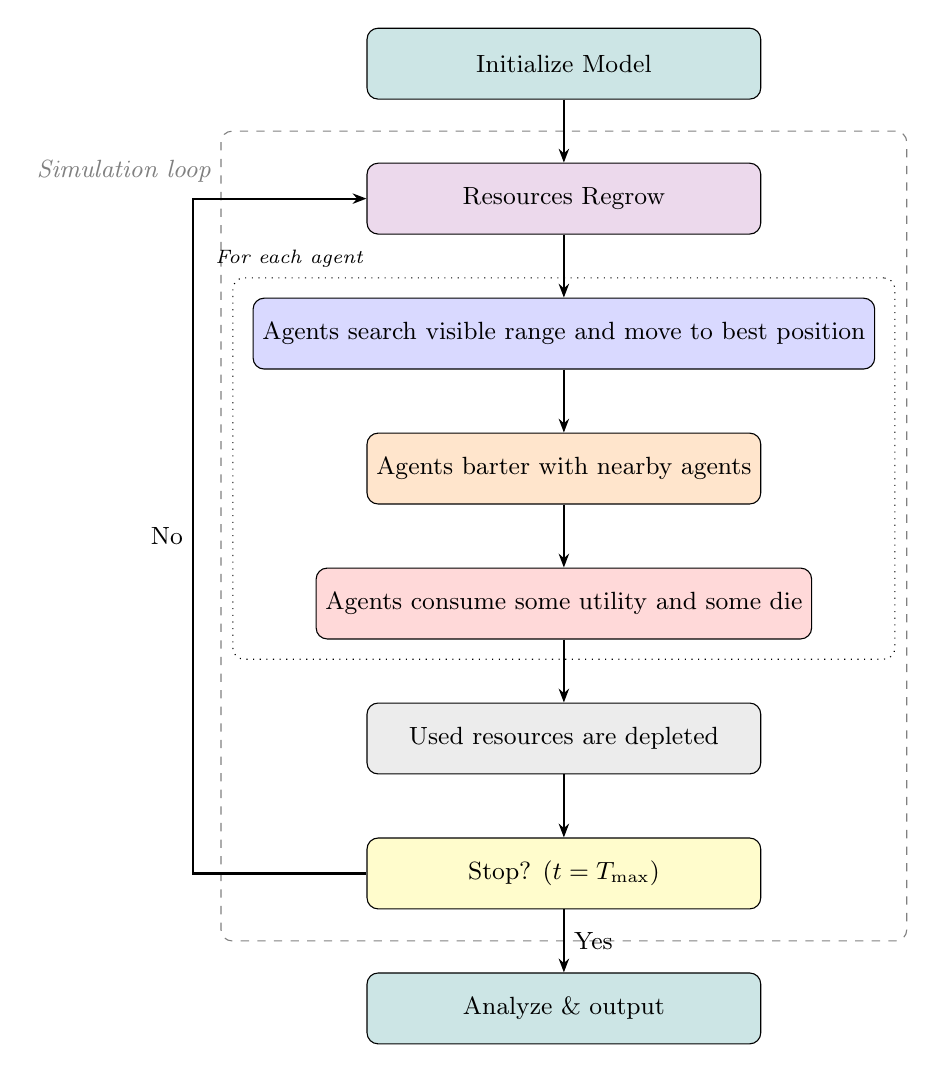
\begin{tikzpicture}[
  node distance=0.8cm,
  box/.style={rectangle, rounded corners, draw, minimum width=5cm, minimum height=0.9cm,
              text centered, font=\small},
  init/.style={box, fill=teal!20},
  envbox/.style={box, fill=violet!15},
  percbox/.style={box, fill=blue!15},
  decbox/.style={box, fill=orange!20},
  actbox/.style={box, fill=red!15},
  databox/.style={box, fill=gray!15},
  stopbox/.style={box, draw, fill=yellow!20},
  outbox/.style={box, fill=teal!20},
  arr/.style={-{Stealth[length=5pt]}, thick},
]

%% Nodes
\node[init]                       (init) {Initialize Model};
\node[envbox,  below=of init]     (env)  {Resources Regrow};
\node[percbox, below=of env]      (perc) {Agents search visible range and move to best position};
\node[decbox,  below=of perc]     (dec)  {Agents barter with nearby agents};
\node[actbox,  below=of dec]      (act)  {Agents consume some utility and some die};
\node[databox, below=of act]      (data) {Used resources are depleted};
\node[stopbox, below=of data]     (stop) {Stop? ($t = T_{\max}$)};
\node[outbox,  below=of stop]     (out)  {Analyze \& output};

%% Arrows (main flow)
\draw[arr] (init) -- (env);
\draw[arr] (env)  -- (perc);
\draw[arr] (perc) -- (dec);
\draw[arr] (dec)  -- (act);
\draw[arr] (act)  -- (data);
\draw[arr] (data) -- (stop);
\draw[arr] (stop) -- node[right]{\small Yes} (out);

%% Loop-back arrow (No)
\draw[arr] (stop.west) -- ++(-2.2,0) |- node[left, pos=0.25]{\small No} (env.west);

%% Dashed boxes for loop containers
\begin{scope}[on background layer]
  \node[draw, dashed, rounded corners, inner sep=0.4cm, gray,
        fit=(env)(perc)(dec)(act)(data)(stop),
        label={[gray, font=\small\itshape]above left:Simulation loop}] {};
  \node[draw, dotted, rounded corners, inner sep=0.25cm, black!100,
        fit=(perc)(dec)(act),
        label={[black!100, font=\scriptsize\itshape]above left:For each agent}] {};
\end{scope}

\end{tikzpicture}
\caption{Agent-based model flowchart.}
\label{fig:model_flow_chart}
\end{figure}


\subsection{Parameters and Initialization}
Parameters
\begin{itemize}
    \item Number of agents
    \item Environment topology: Initialized as a function
    \item Resource regrowth rate: Initialized as a scalar [0,1] where 1 is 100\% regrowth
    \item Agent vision: initialized as integer radius they can see
    \item Agent metabolic rate: How much their utility is depleted per time-step
    \item Agent preferences: Initialized as a list of relative preferences for each good
\end{itemize}

\subsection{Assessment and Outcome Measures}
I would like to track inequality, death rate, and the cost effectiveness of different interventions. I would also like to track supply and demand and see if trade is able to reach equilibrium or if there will be pockets of inefficiency. I plan to track inequality by looking at the distribution of wealth in the economy over time, and I would like to conduct a cost-benefit analysis on different interventions by comparing utility distributions with and without the intervention. 

\subsection{Parameter Exploration}
I plan on exploring parameter space for as many parameters as I computationally can. I am most interested in resource regrowth rate, metabolic rate, and maybe environment topology. The regrowth rate is nicely between zero and one, but the metabolic rate is just a number. However, metabolic rate should likely be positive and low enough that all agents don't just simply die. Sampling the function used to generate the resource gradients will be more challenging, but I think I will sample variations of a reasonable functional form. I think it would be interesting to compare steeper environments with more gradual resource gradients.

\section{Questions and Challenges}
One question I have is how to handle the resource function for multiple goods. I was thinking that I could add multiple resource functions to the environment.

\section{Code}
Check the attached Jupyter notebook for the model code as of writing this, or check my GitHub repository for updated code.
\newline

\centering
\href{https://github.com/Zeke-CE/CSCS530Project-repo.git}{Click here to view model repository}



\clearpage
\bibliographystyle{plain}
\bibliography{references}

\end{document}

